\documentclass[9pt,aspectratio=169,hyperref=colorlinks]{beamer}

\usetheme{Goettingen}
\usecolortheme{crane}
\usefonttheme{professionalfonts}
\setbeamercolor{item}{fg=black}
\setbeamertemplate{itemize items}[circle]
\setbeamertemplate{footline}[frame number]

\usepackage{xeCJK}
% \setCJKmainfont{Noto Serif CJK SC}
% \setCJKsansfont{Noto Sans CJK SC}
% \setCJKmonofont{Noto Sans Mono CJK SC}

\usepackage{calligra}
\usepackage{mathtools}
\usepackage{minted}
\usepackage{physics}
\usepackage{ragged2e}
\justifying\let\raggedright\justifying
\usepackage{tikz}
\usebackgroundtemplate{\tikz\node[opacity=0.15]{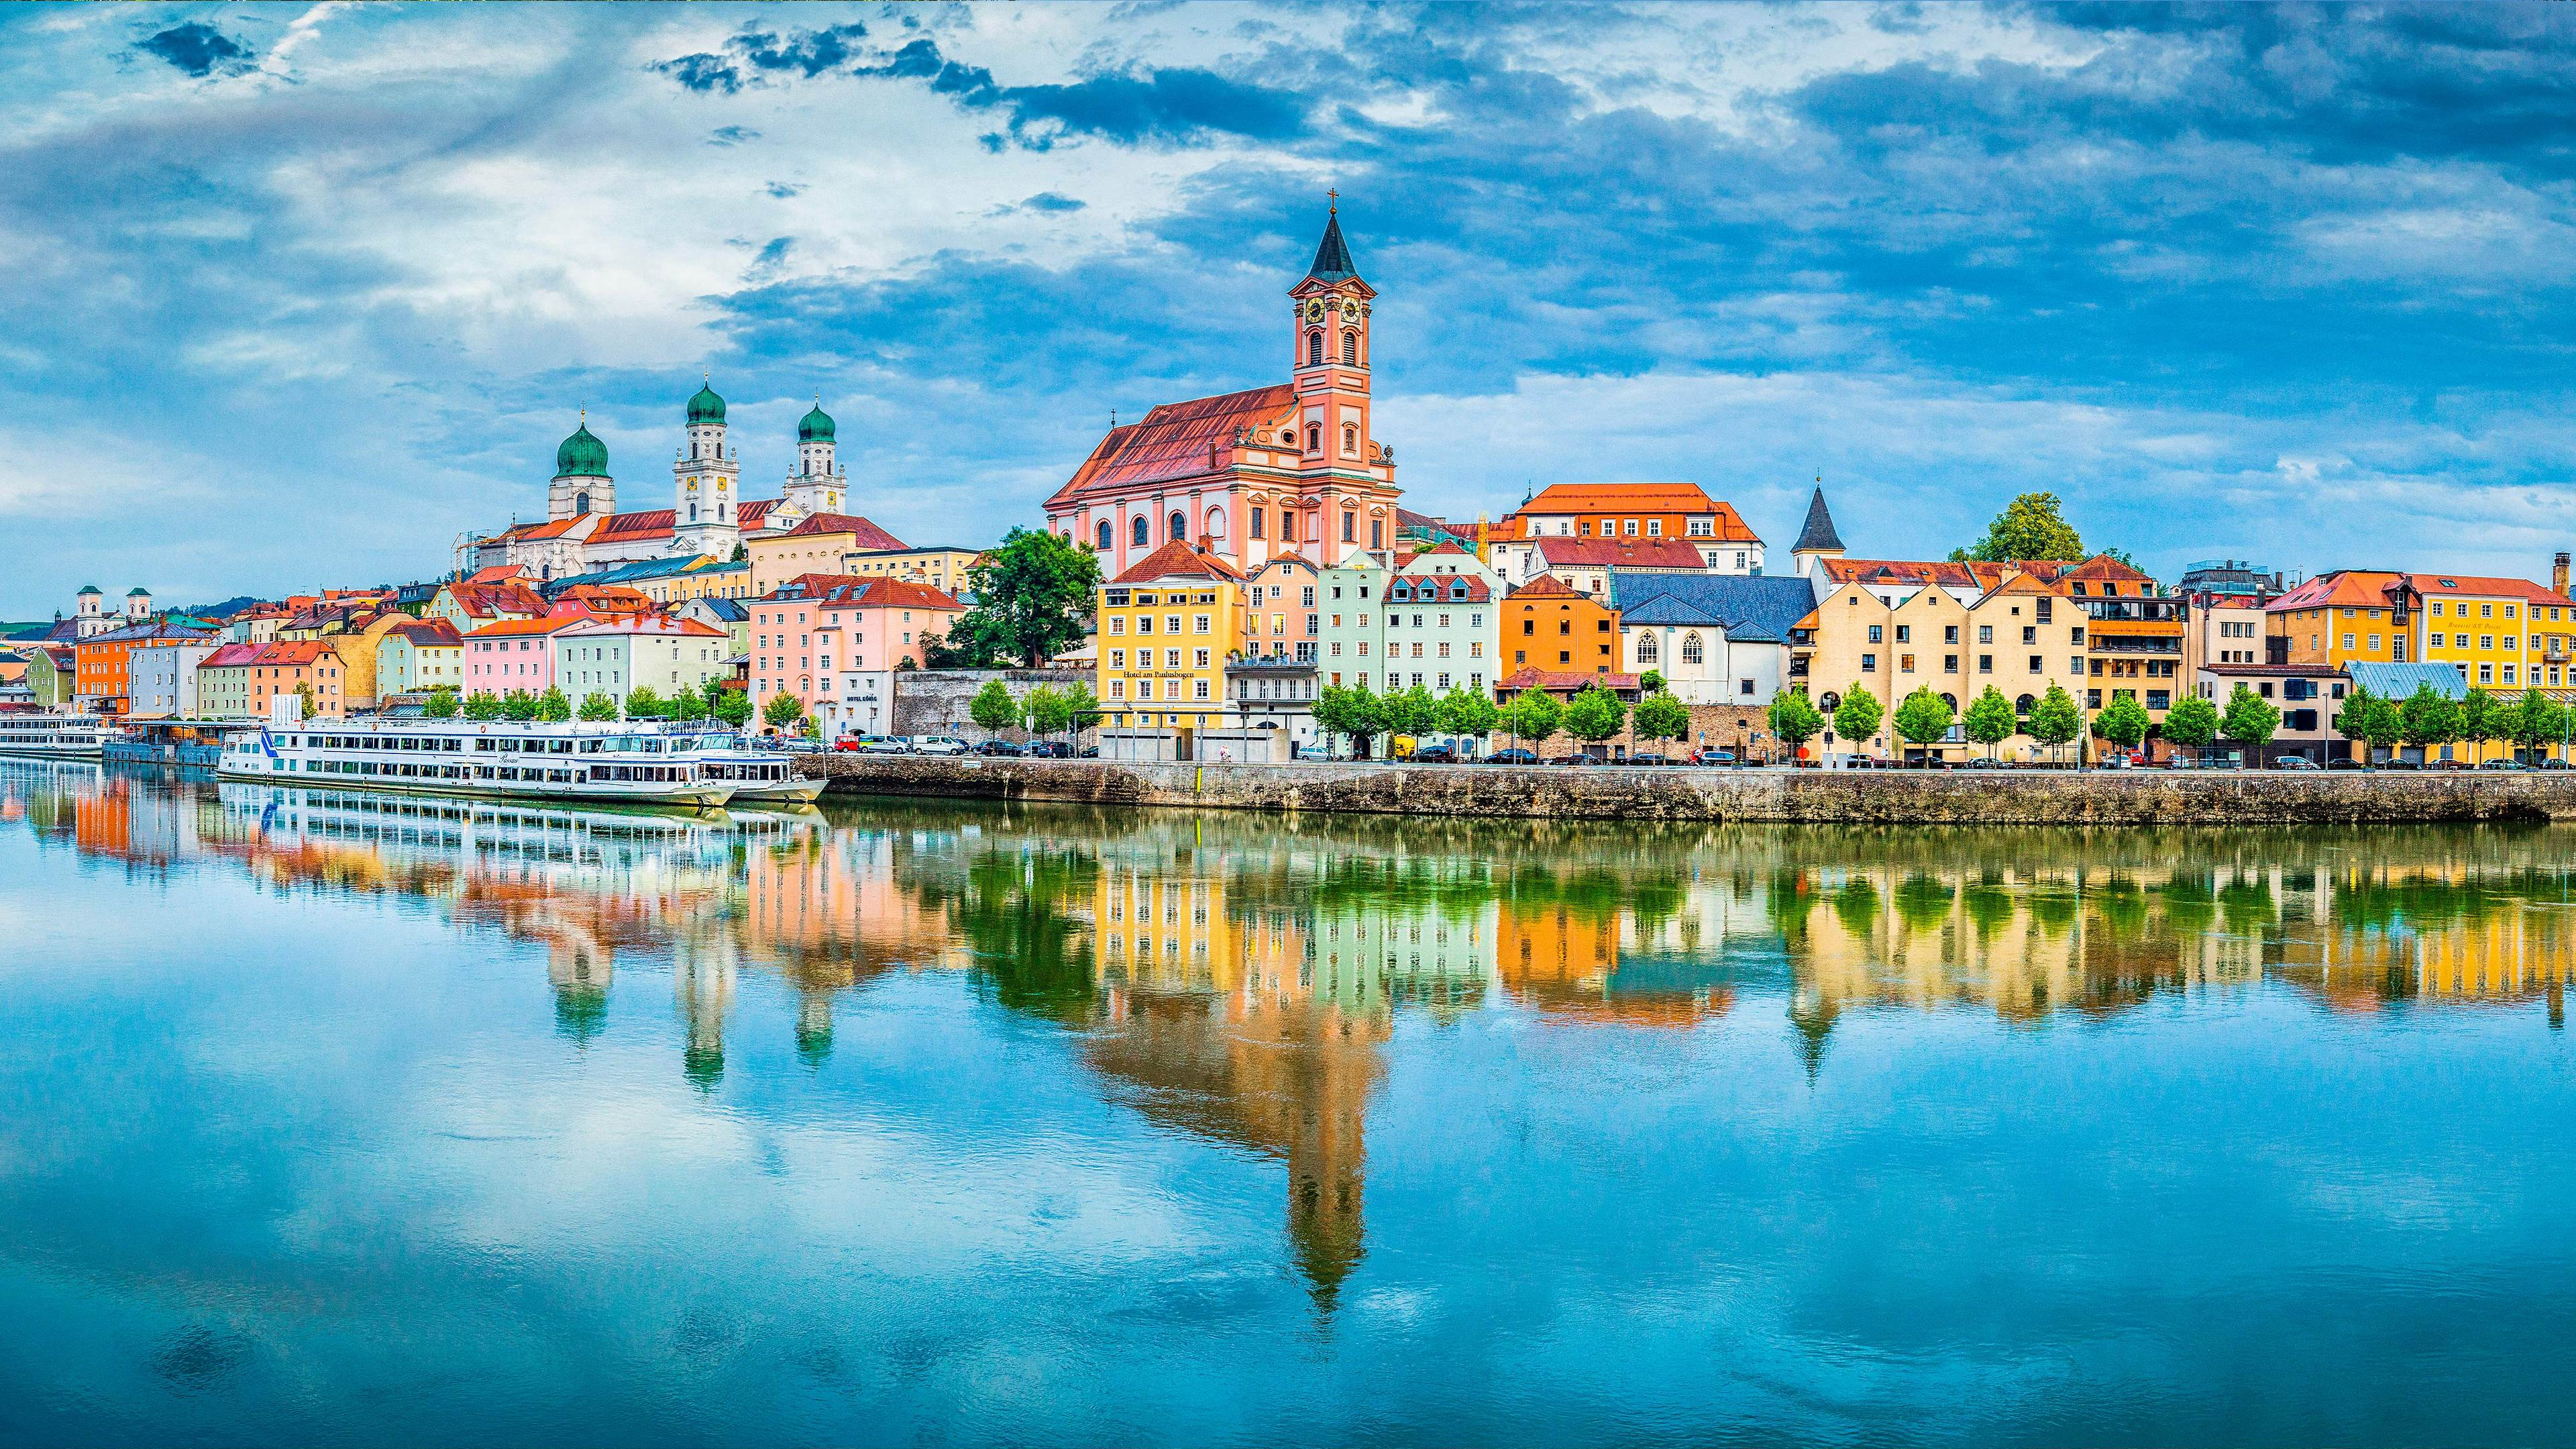
\includegraphics[width=\paperwidth]{CV/figs/background.jpeg}};}

\title{Personal Statement}
\institute{College of Science, Hohai University}
\author{Feng Zhe / 冯哲}
\date{July 7, 2023}

\begin{document}

\frame{\titlepage}

\section{Introduction}
\begin{frame}{Introduction}
    \begin{itemize}
        \item Feng Zhe / 冯哲
        \item Undergraduate, College of Science, Hohai University, Nanjing, China
        \item E-mail: \href{mailto:2010020129@hhu.edu.cn}{2010020129@hhu.edu.cn} / \href{mailto:ph3n92h3@hhu.edu.cn}{ph3n92h3@hhu.edu.cn}
        \item Homepage: \href{https://ph3n92h3.github.io}{https://ph3n92h3.github.io}
    \end{itemize}
\end{frame}

\section{Education Background}
\begin{frame}{Education Background}
    \textbf{Hohai University} \hfill Sept. 2020 - Present

    \textit{B.Sc in Physics \hfill GPA: 4.86/5.00, ranking 1/57}

    \begin{itemize}
        \item Mechanics: 92, Thermal Physics: 95, Electromagnetism: 94, Fundamental Optics: 91
        \item Method of Mathematical Physics: 99
        \item Theoretical Mechanics: 93
        \item Electrodynamics: 97
        \item Thermodynamics and Statistical Mechanics: 97
        \item Quantum Mechanics: 99, Advanced Quantum Mechanics: 93
        \item Solid-state Physics: 94, Semiconductor Physics: 95
    \end{itemize}
\end{frame}

\section{Research Experience}
\begin{frame}{Research Experience: Publications}
    \begin{enumerate}
        \item Charged anisotropic white dwarfs in $f\left({R}, {T}\right)$ gravity, Zhe Feng, \href{https://arxiv.org/abs/2210.01574}{arxiv:2210.01574[gr-qc]} \[S = \int \dd[4]{x} \sqrt{-g} \qty[\underbrace{\frac{1}{16 \pi} f(R, T)}_{\mathcal{L}_g} + \overbrace{p_r}^{\mathcal{L}_m} + \underbrace{j^a A_a - \frac{1}{16 \pi} F_{ab} F^{ab}}_{\mathcal{L}_e}]\]
        \item Slow-roll inflation in $f\left(R, T, R_{ab}T^{ab}\right)$ gravity, Zhe Feng, \href{https://arxiv.org/abs/2211.13233}{arxiv:2211.13233[gr-qc]} \[S = \int \dd[4]{x} \sqrt{-g} \qty[\underbrace{\frac{f\qty(R, T, R_{ab}T^{ab})}{2 \kappa}}_{\mathcal{L}_g} \overbrace{- \frac{1}{2} g^{ab} \nabla_{a} \phi \nabla_{b} \phi - V(\phi)}^{\mathcal{L}_m}]\]
    \end{enumerate}
\end{frame}

\begin{frame}{Research Experience: General Relativity and Quantum Cosmology}
    \textbf{General Relativity and Quantum Cosmology} \hfill Feb. 2022 - Present

    \smallskip \quad \textit{Modified Gravity and Astrophysics}

    \textbf{Z. Feng}, \textit{Charged anisotropic white dwarfs in $f\left({R}, {T}\right)$ gravity}, \href{https://arxiv.org/abs/2210.01574}{arxiv:2210.01574[gr-qc]}

    \[S = \int \dd[4]{x} \sqrt{-g} \qty[\underbrace{\frac{1}{16 \pi} f(R, T)}_{\mathcal{L}_g} + \overbrace{p_r}^{\mathcal{L}_m} + \underbrace{j^a A_a - \frac{1}{16 \pi} F_{ab} F^{ab}}_{\mathcal{L}_e}]\]

    \begin{itemize}
        \item In the context of $f(R, T) = R + 2 \beta T$ gravity, where $R$ is the Ricci scalar and $T$ is the trace of the energy-momentum tensor, the equilibrium structure of charged anisotropic white dwarfs (WDs) is studied. The stellar equations for the general case are derived and numerical solutions are found for the Chandrasekhar equation of state (EoS) and a charge density distribution proportional to the energy density $\rho_{ch} = \alpha \rho$. By adjusting different parameters, the properties of the solutions under various conditions are compared. Most importantly, by going beyond the trivial WD in GR in various ways, the solutions may exhibit super-Chandrasekhar behavior. This paper is a study of a WD structure, and the results obtained may have a contrasting effect on astronomical observations such as superluminous type Ia supernovae.
    \end{itemize}
\end{frame}

\begin{frame}{Research Experience: General Relativity and Quantum Cosmology}
    \textbf{General Relativity and Quantum Cosmology} \hfill Feb. 2022 - Present

    \smallskip \quad \textit{Modified Gravity and Cosmology}

    \textbf{Z. Feng}, \textit{Slow-roll inflation in $f\left(R, T, R_{ab}T^{ab}\right)$ gravity}, \href{https://arxiv.org/abs/2211.13233}{arxiv:2211.13233[gr-qc]}

    \[S = \int \dd[4]{x} \sqrt{-g} \qty[\underbrace{\frac{f\qty(R, T, R_{ab}T^{ab})}{2 \kappa}}_{\mathcal{L}_g} \overbrace{- \frac{1}{2} g^{ab} \nabla_{a} \phi \nabla_{b} \phi - V(\phi)}^{\mathcal{L}_m}]\]

    \begin{itemize}
        \item In the framework of $f\left(R, T, R_{ab}T^{ab}\right)$ gravity theory, the slow-roll approximation of the cosmic inflation is investigated, where $T$ is the trace of the energy-momentum tensor $T^{ab}$, $R$ and $R_{ab}$ are the Ricci scalar and tensor, respectively. After obtaining the equations of motion of the gravitational field from the action principle in the spatially flat FLRW metric, the fundamental equations of this theory are received by introducing the inflation scalar field as the matter and taking into account only the minimum curvature-inflation coupling term. Remarkably, after taking the slow-roll approximation, the identical equations as in $f(R, T)$ gravity with a $RT$ mixing term are derived. Several potentials of interest in different domains are evaluated individually, calculating the slow-roll parameter and the e-folding number $N$. Finally, we analyze the behavior of the inflation scalar field under perturbation while ignoring the effect of metric perturbations. This research complements the slow-roll inflation in the modified theory of gravity.
    \end{itemize}
\end{frame}

\begin{frame}{Research Experience: Condensed Matter - Materials Science}
    \medskip \textbf{Condensed Matter - Materials Science} \hfill Sept. 2021 - Present

    \quad \textit{Miniaturized Wavelength-Resolvable Photodetector Based on Fabry-P\'{e}rot Multilayer Film / Si Structure}

    \hfill \textit{Prof. Zhibin Shao(HHU)}

    \begin{itemize}
        \item Hohai University Innovation Training Project for Undergraduates \textit{Excellent Completion}
        \item The absorption spectrum of silicon is not selective to the wavelength of light, which makes it difficult for existing photodetectors to achieve spectral resolution, which limits the application scenarios of photodetectors. The Fabry-P\'{e}rot multilayer film is expected to solve this problem due to its high flexibility and strong wavelength selection performance. By coupling the Fabry-P\'{e}rot multilayer film with silicon-based semiconductors, Wavelength selection can be performed while light detection is performed, thereby achieving wavelength resolution.
        \item Traditional large-scale, fixed spectrometers usually require long optical paths and wide receiving surfaces, which are difficult to meet the application requirements of timeliness, portability, and miniaturization. Photodetectors are based on electrode layers and single crystal silicon. The photoelectric characteristics are based on the intrinsic properties of semiconductors and do not depend on long optical paths and wide receiving surfaces. Applying them to spectral resolution can solve the size limitation of traditional spectrometers.
    \end{itemize}
\end{frame}

\begin{frame}{Research Experience: Condensed Matter - Materials Science}
    \medskip \textbf{Condensed Matter - Materials Science} \hfill Sept. 2021 - Present

    \quad \textit{Miniaturized Wavelength-Resolvable Photodetector Based on Fabry-P\'{e}rot Multilayer Film / Si Structure}

    \hfill \textit{Prof. Zhibin Shao(HHU)}

    \begin{itemize}
        \item Hohai University Innovation Training Project for Undergraduates \textit{Excellent Completion}
    \end{itemize}

    \begin{figure}
        \centering
        \includegraphics[scale=0.12]{CV/figs/Miniaturized Wavelength-Resolvable Photodetector Based on Fabry-Perot Multilayer Film ⁄ Si Structure.png}
    \end{figure}
\end{frame}

\begin{frame}{Research Experience: Condensed Matter - Materials Science}
    \medskip \textbf{Condensed Matter - Materials Science} \hfill Apr. 2022 - May 2023

    \quad \textit{Laser Etching-Assisted Patterning of Silicon Micro-Nano Structures}

    \hfill \textit{Prof. Zhibin Shao(HHU)}

    \begin{itemize}
        \item Hohai University Innovation Training Project for Undergraduates \textit{Excellent Completion}
        \item Laser has the characteristics of good monochromaticity, good directionality, high precision, and high designability. Compared with other preparation methods of micro-nano structure materials, laser processing has the advantages of simple equipment, high arbitrariness, and easy adjustment of parameters. It is of great significance to study the application of laser etching in the preparation of silicon micro-nano structures.
        \item In the production of photovoltaic cells, surface texturing technology is used to prepare silicon micro-nano structures to improve the light absorption rate and photoelectric conversion efficiency of the panel. However, this technology also makes silicon-based photovoltaic panels present a single dark color, reducing the aesthetics of photovoltaic panels. By precisely controlling the size and position of silicon micro-nano structures, local optical properties of silicon wafers can be controlled, which is expected to realize the preparation of patterned photovoltaic panels and promote the development of the decorative solar industry.
    \end{itemize}
\end{frame}

\begin{frame}{Research Experience: Condensed Matter - Materials Science}
    \medskip \textbf{Condensed Matter - Materials Science} \hfill Apr. 2022 - May 2023

    \quad \textit{Laser Etching-Assisted Patterning of Silicon Micro-Nano Structures}

    \hfill \textit{Prof. Zhibin Shao(HHU)}

    \begin{itemize}
        \item Hohai University Innovation Training Project for Undergraduates \textit{Excellent Completion}
    \end{itemize}

    \begin{figure}
        \centering
        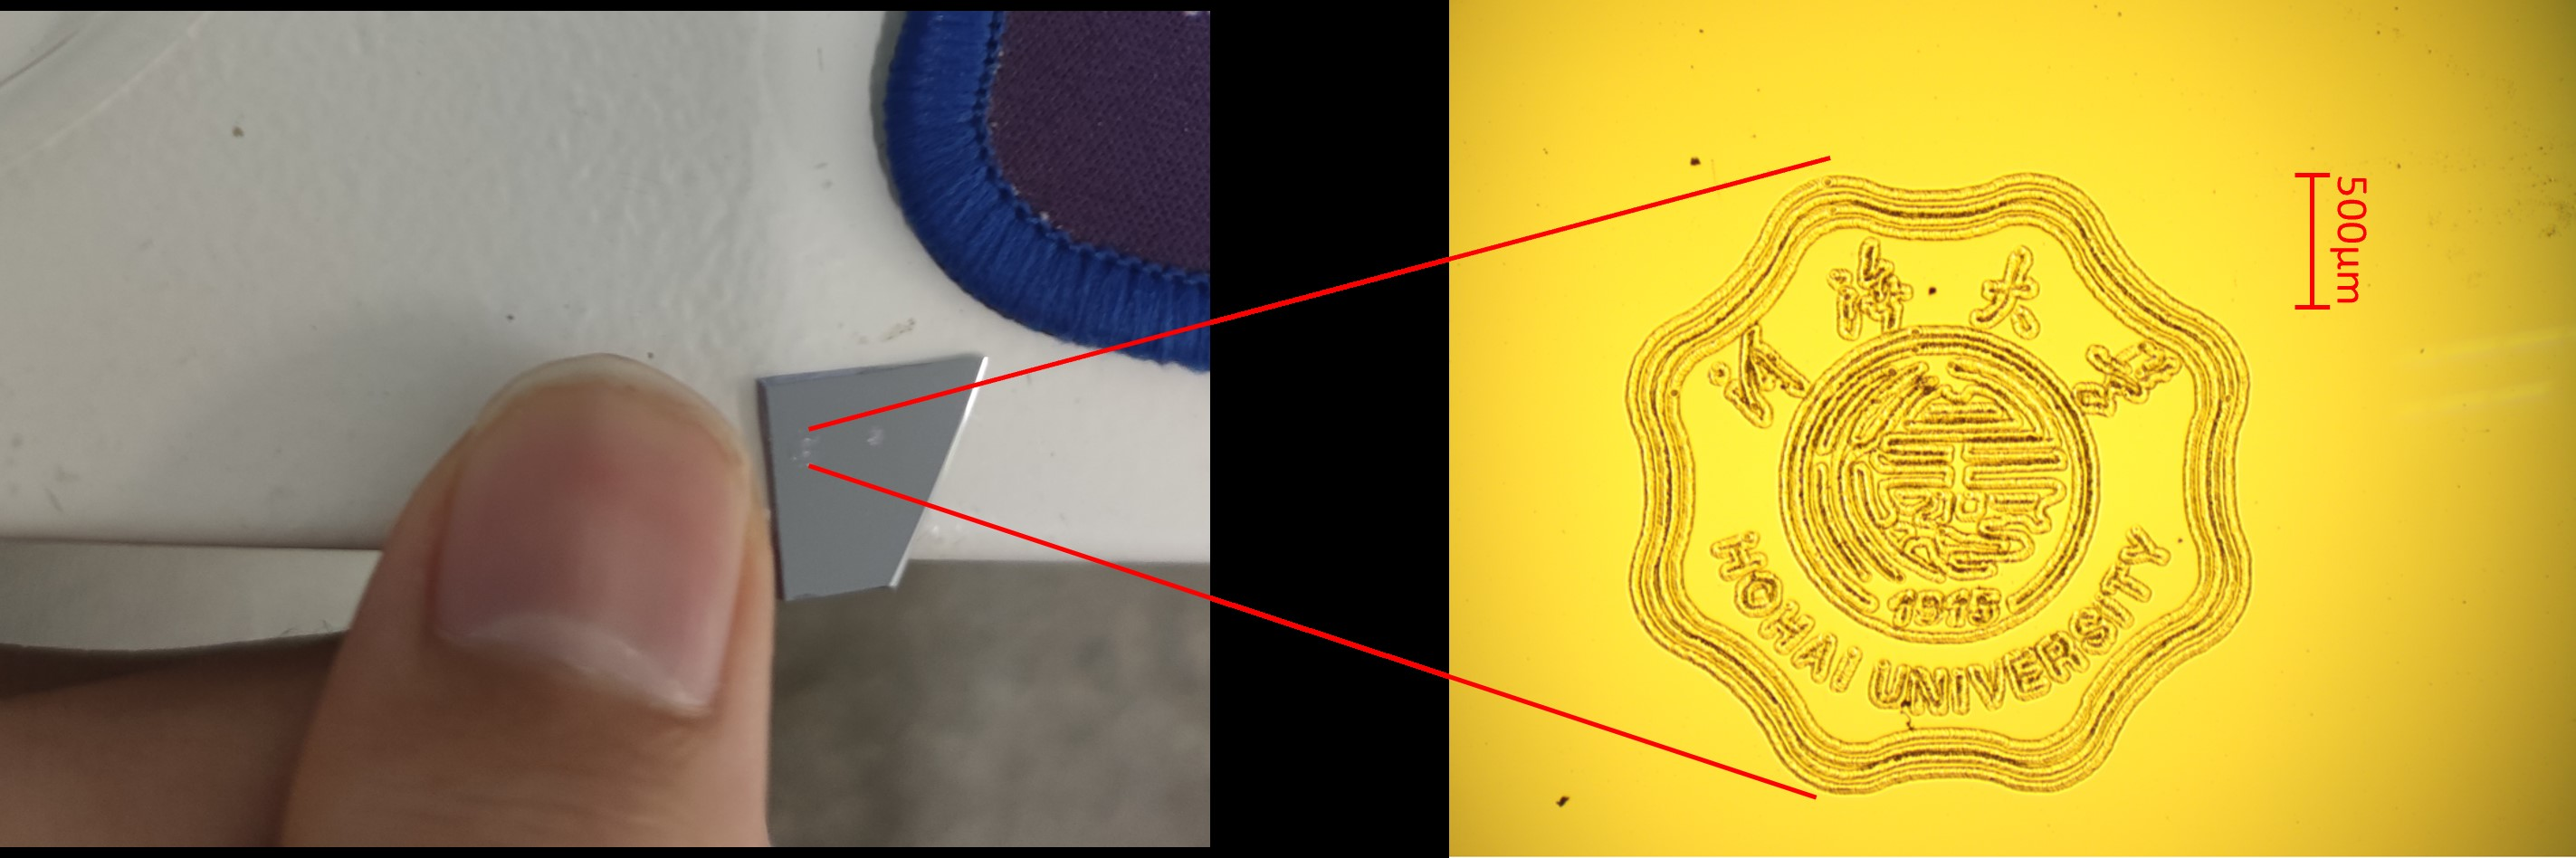
\includegraphics[scale=0.59]{CV/figs/Laser Etching-Assisted Patterning of Silicon Micro-Nano Structures.png}
    \end{figure}
\end{frame}

\section{Research Interests}
\begin{frame}{Research Interests}
    High Energy Physics - Theory (hep-th)
    \begin{itemize}
        \item string theory
        \item supersymmetric field theory
        \item scattering amplitude
    \end{itemize}

    General Relativity and Quantum Cosmology (gr-qc)
    \begin{itemize}
        \item gravity theory
        \item cosmological inflation, cosmological perturbation
        \item black hole, compact star
    \end{itemize}
\end{frame}

\section{Computer Science}
\begin{frame}{Computer Science}
    \href{https://www.wolfram.com/mathematica/}{Wolfram Mathematica}
    \begin{itemize}
        \item Numerical solution of the equilibrium structure of compact stars
        \item Calculations of gravitational theory using \href{http://xact.es/index.html}{xAct}
        \item Modeling calculations using optical thin film theory
    \end{itemize}

    \href{https://archlinux.org}{Arch Linux}
    \begin{itemize}
        \item use on a daily base
    \end{itemize}

    \href{https://www.latex-project.org}{\LaTeX}
    \begin{itemize}
        \item all of my papers, notes, slides...
    \end{itemize}
\end{frame}

\begin{frame}{Computer Science}
    \begin{itemize}
        \item \href{https://www.wolfram.com/mathematica/}{Wolfram Mathematica}: Numerical solution of the equilibrium structure of compact stars
    \end{itemize}

    \begin{figure}
        \centering
        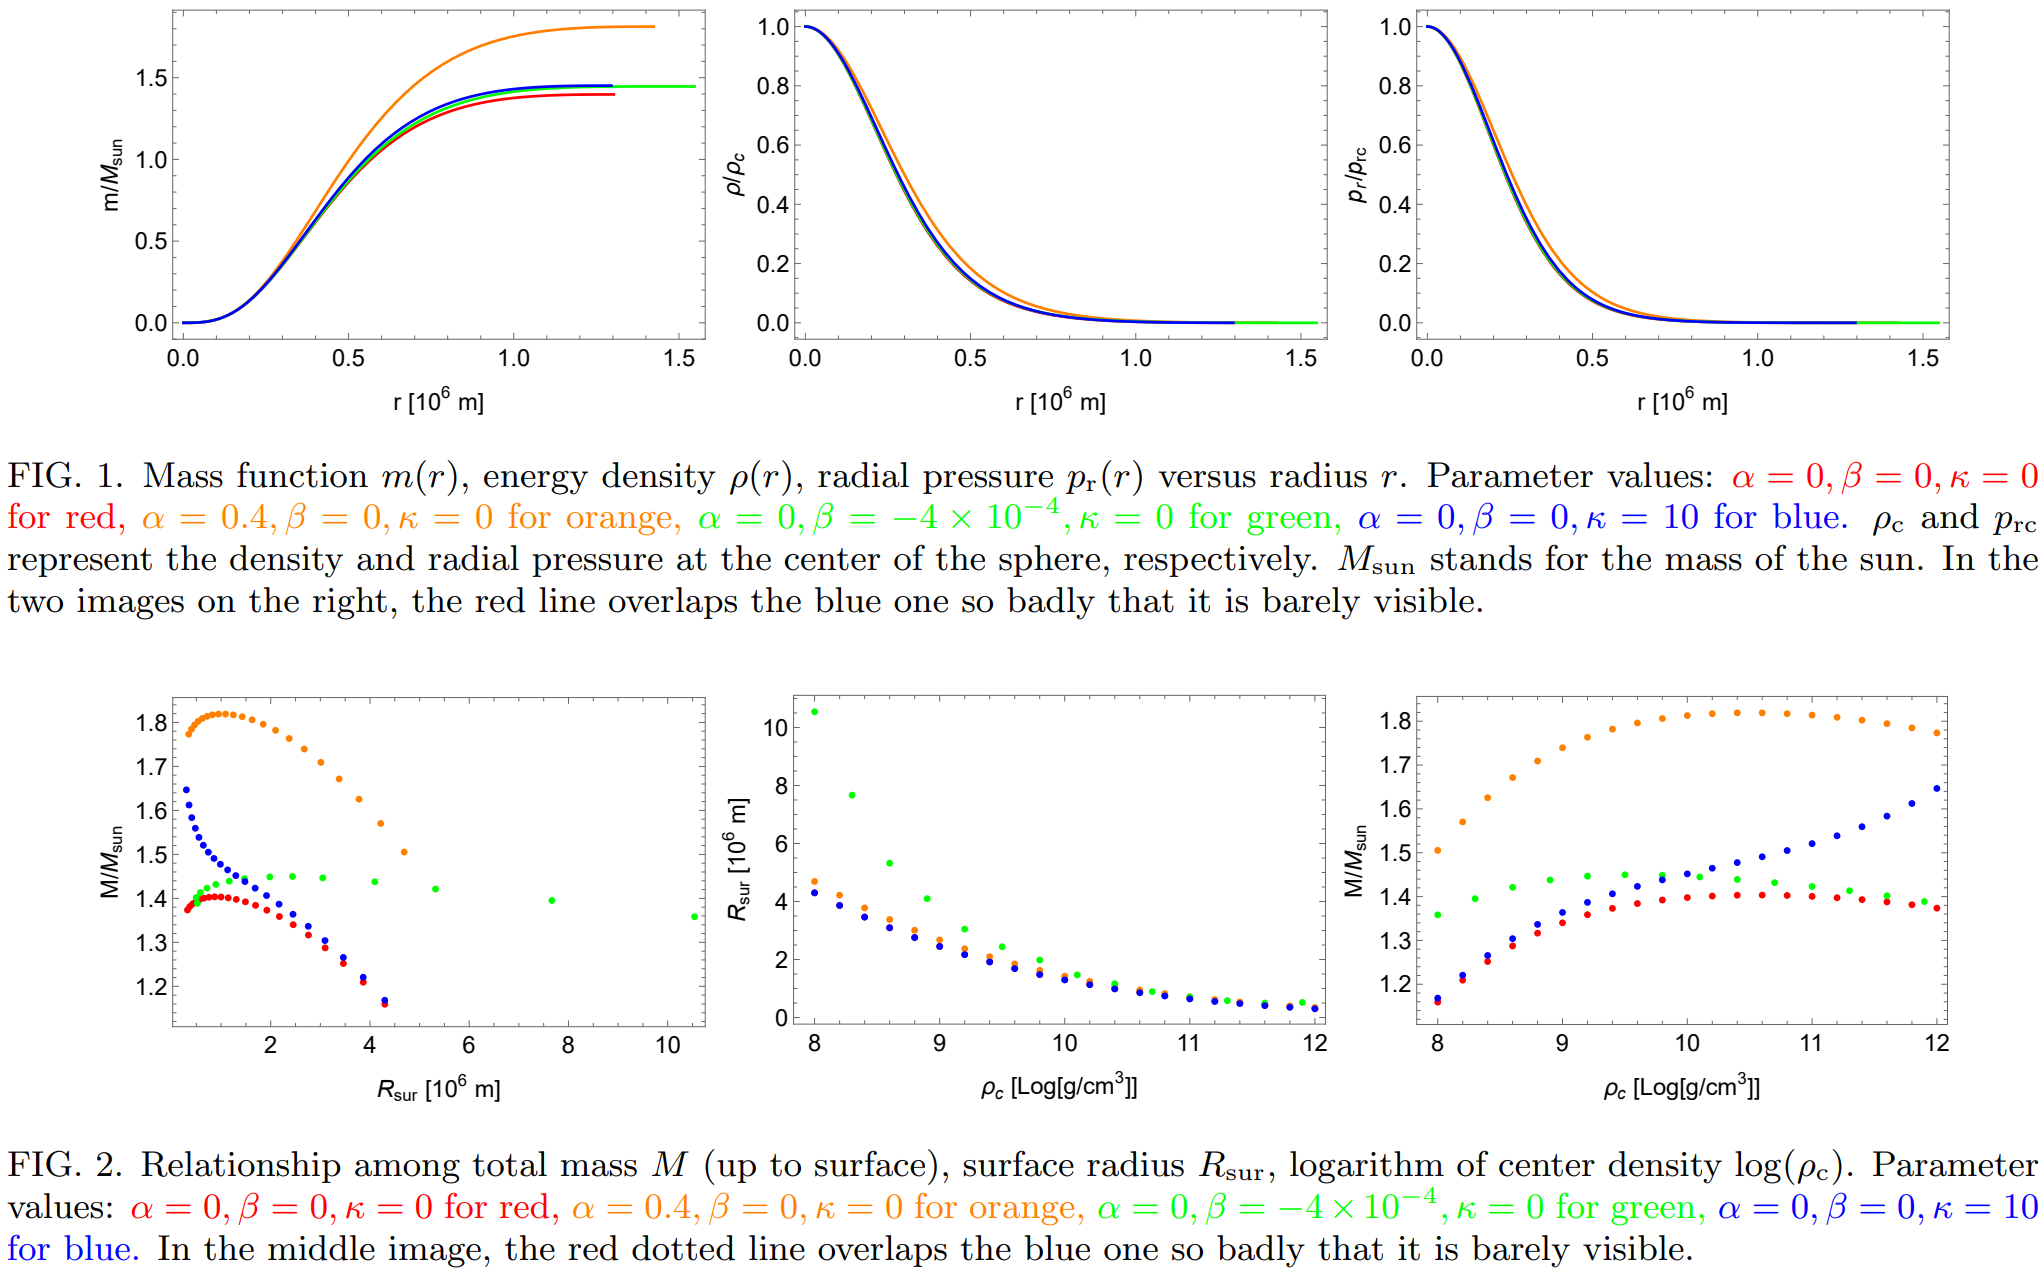
\includegraphics[scale=0.2]{CV/figs/2210.01574.png}
    \end{figure}
\end{frame}

\begin{frame}{Computer Science}
    \begin{itemize}
        \item \href{https://www.wolfram.com/mathematica/}{Wolfram Mathematica}: Calculations of gravitational theory using \href{http://xact.es/index.html}{xAct}
    \end{itemize}

    \begin{figure}
        \centering
        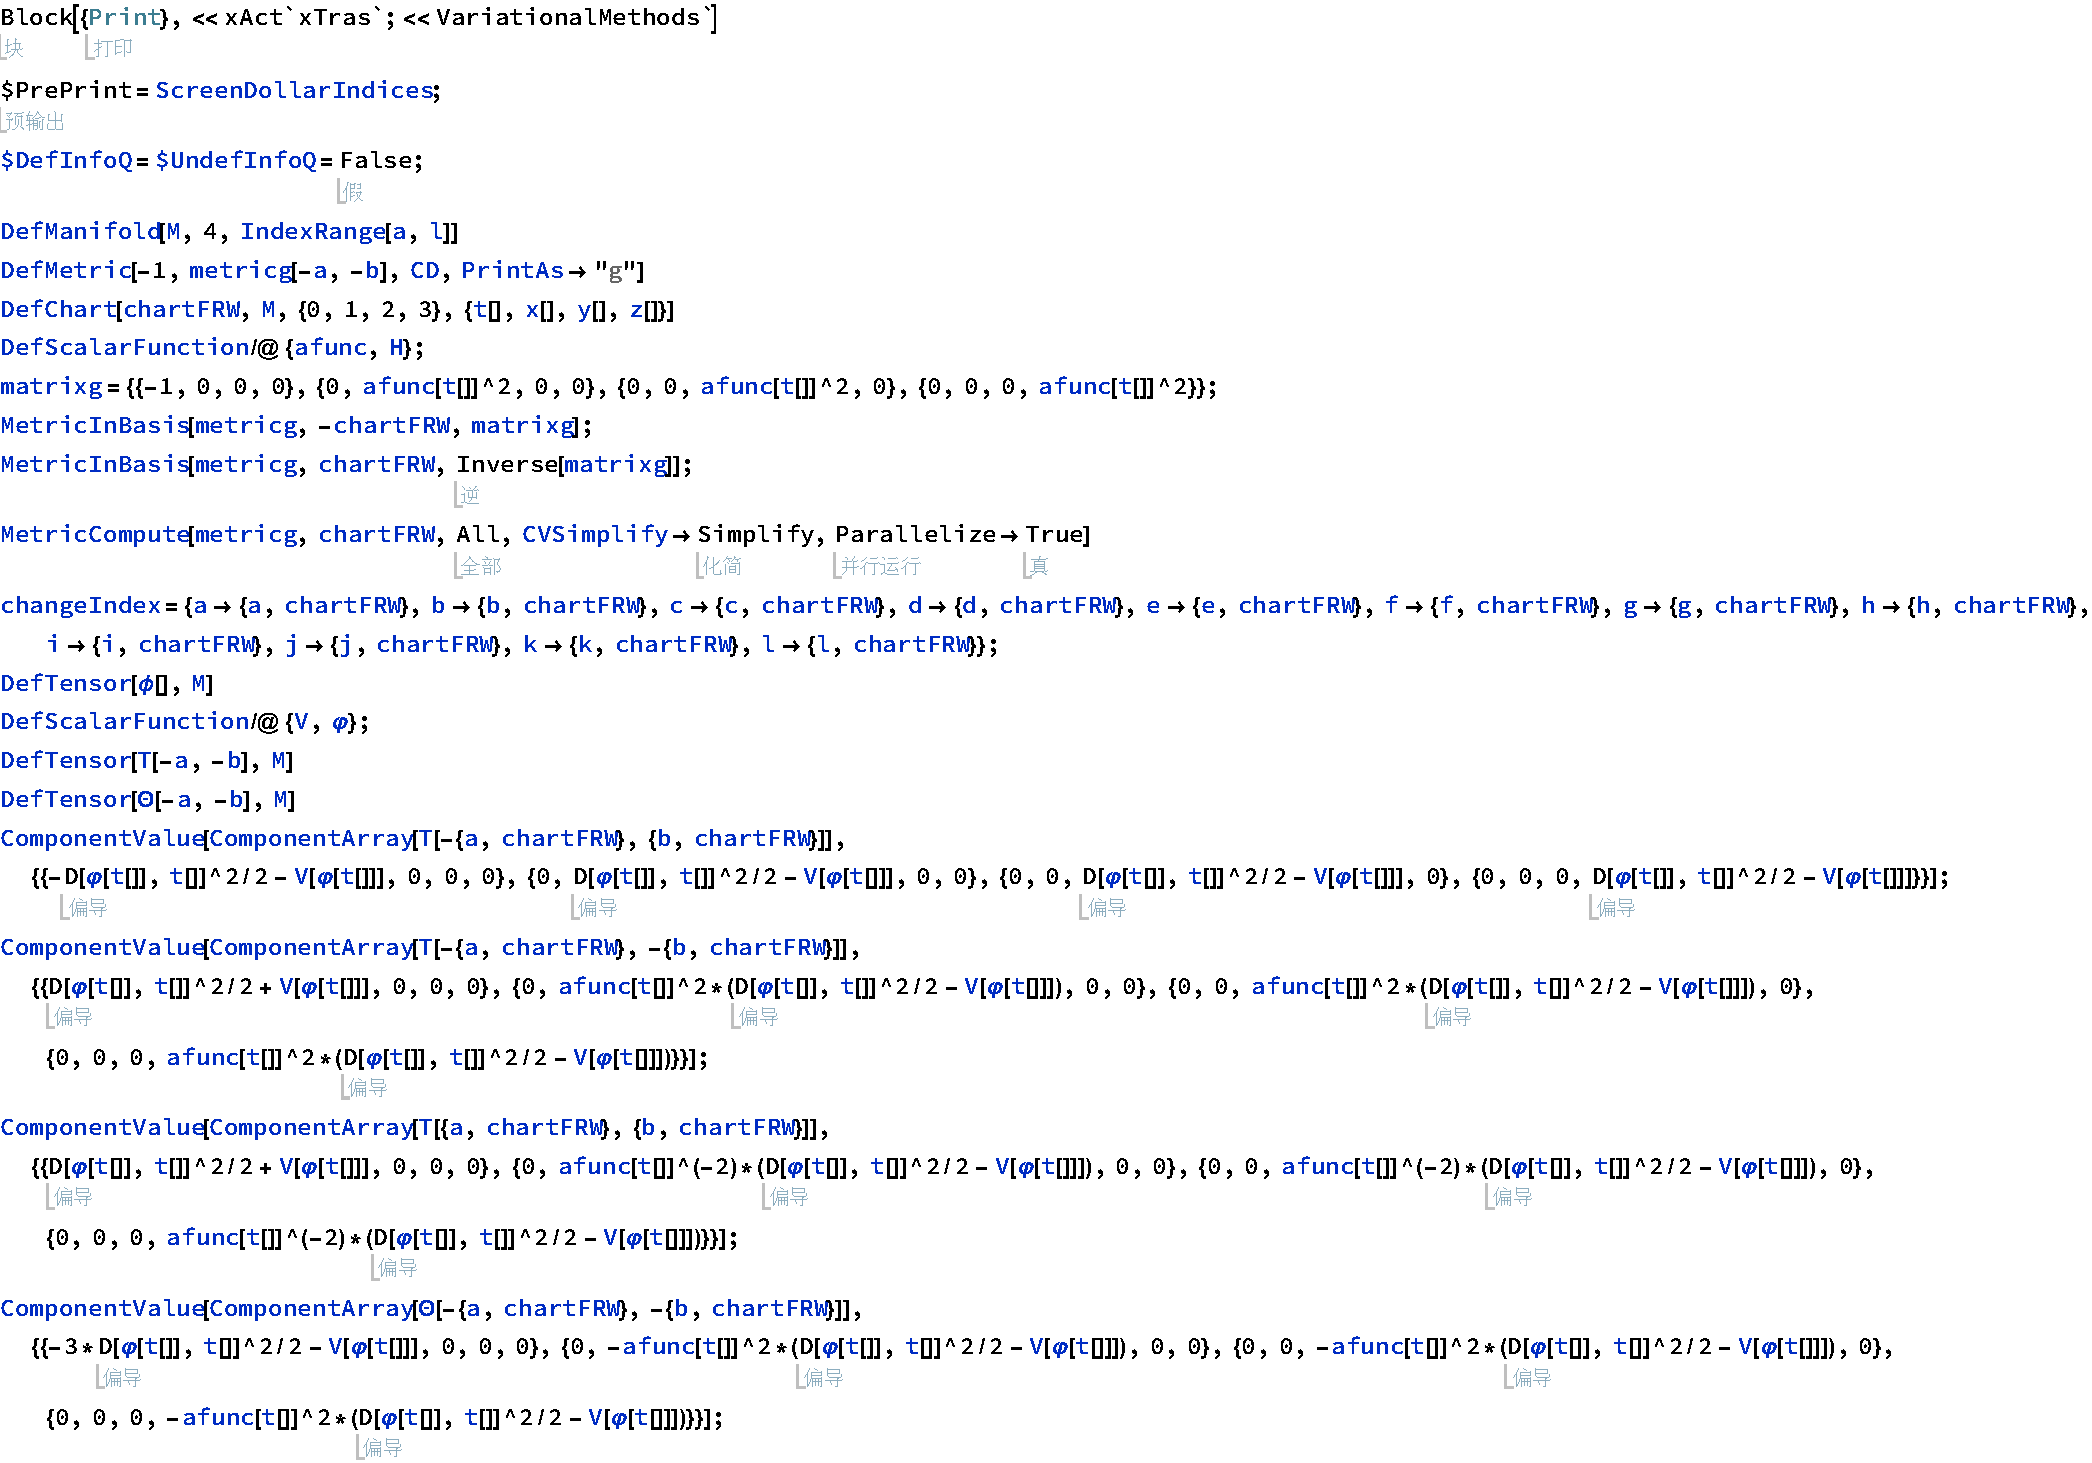
\includegraphics[scale=0.29]{CV/figs/2211.13233.1.pdf}
    \end{figure}
\end{frame}

\begin{frame}{Computer Science}
    \begin{itemize}
        \item \href{https://www.wolfram.com/mathematica/}{Wolfram Mathematica}: Calculations of gravitational theory using \href{http://xact.es/index.html}{xAct}
    \end{itemize}

    \begin{figure}
        \centering
        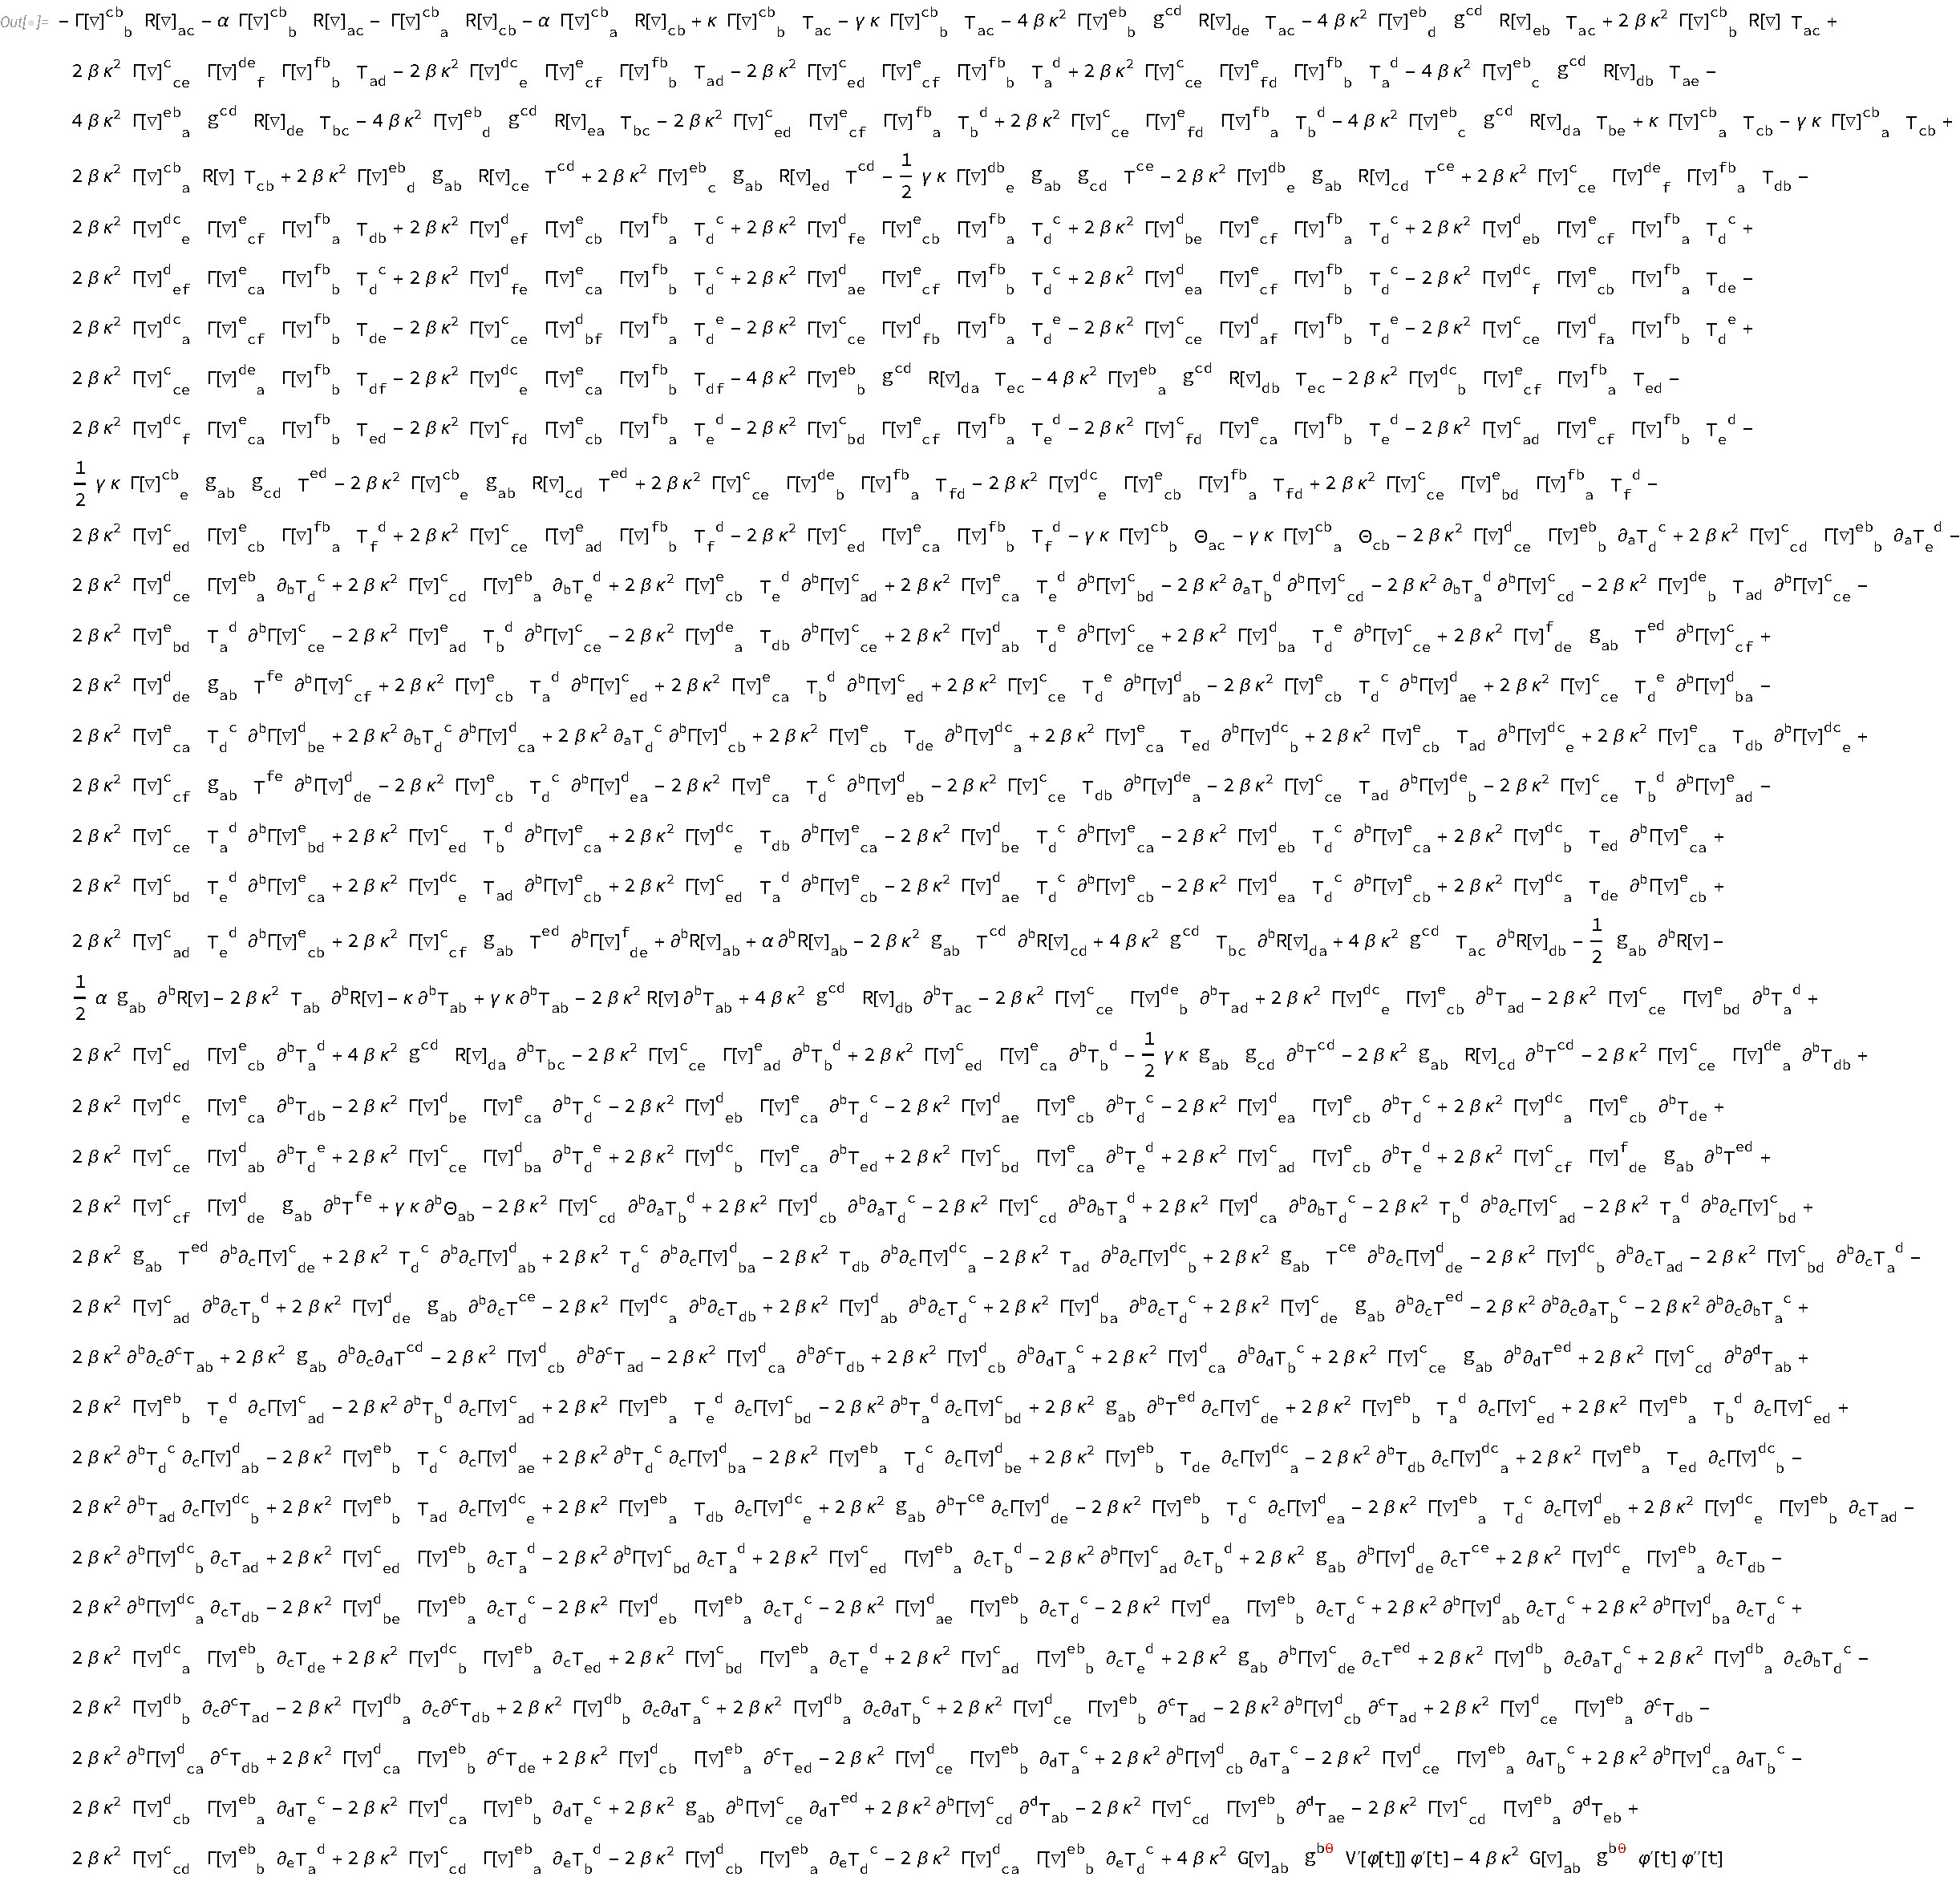
\includegraphics[scale=0.32]{CV/figs/2211.13233.2.pdf}
    \end{figure}
\end{frame}

\begin{frame}{Computer Science}
    \begin{itemize}
        \item \href{https://www.wolfram.com/mathematica/}{Wolfram Mathematica}: Modeling calculations using optical thin film theory
    \end{itemize}

    \begin{figure}
        \centering
        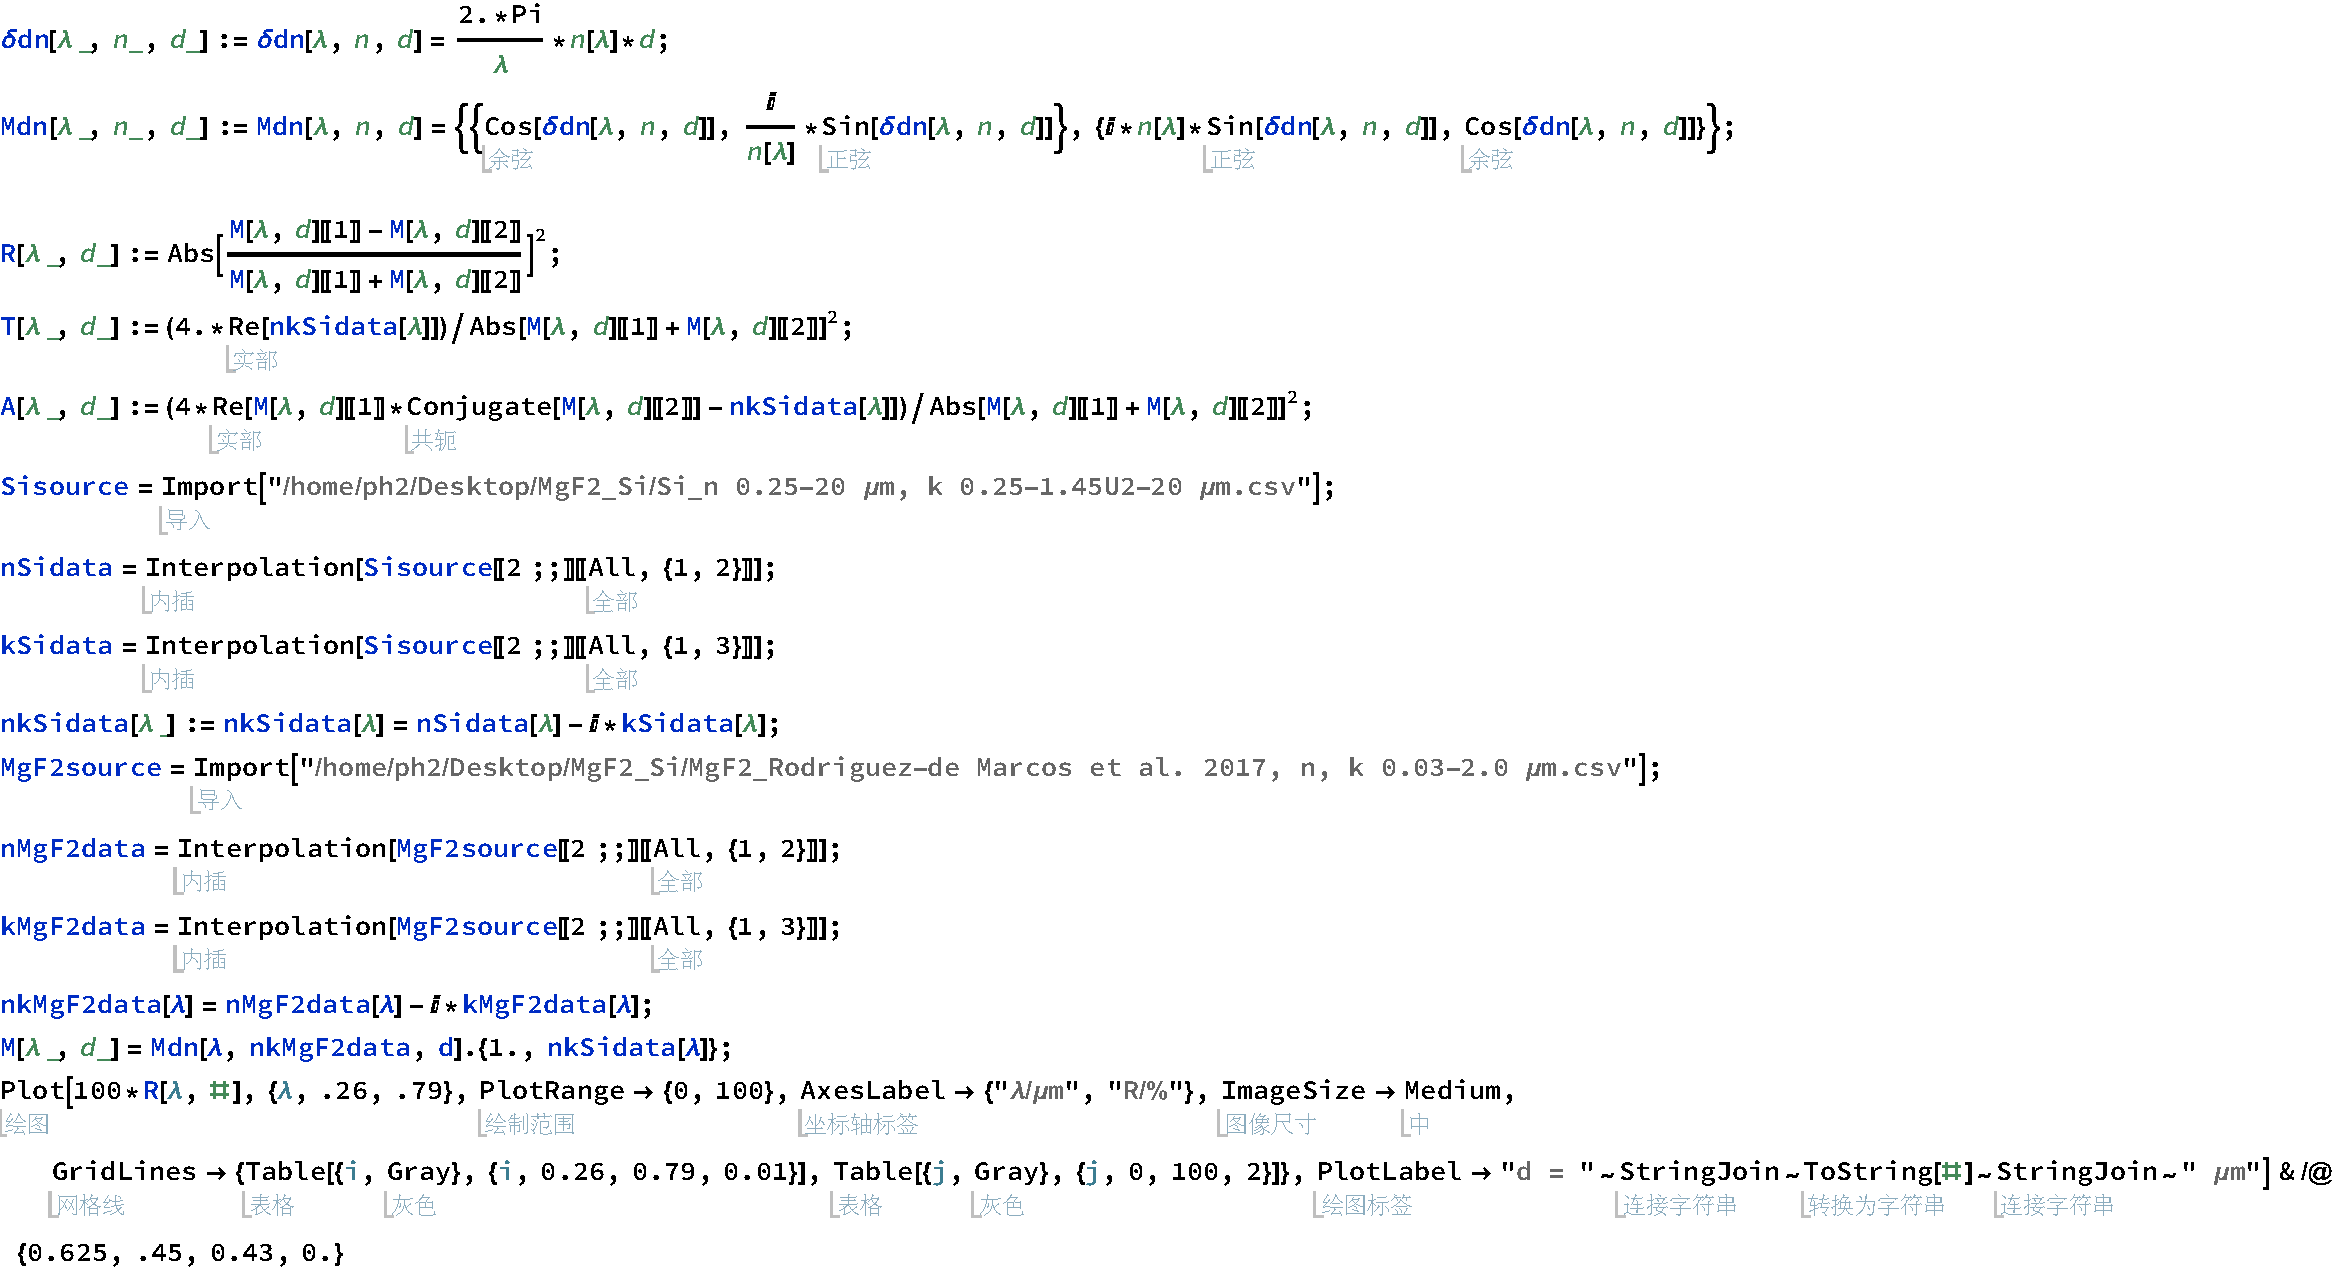
\includegraphics[scale=0.31]{CV/figs/3.1.pdf}
    \end{figure}
\end{frame}

\begin{frame}{Computer Science}
    \begin{itemize}
        \item \href{https://www.wolfram.com/mathematica/}{Wolfram Mathematica}: Modeling calculations using optical thin film theory
    \end{itemize}

    \begin{figure}
        \centering
        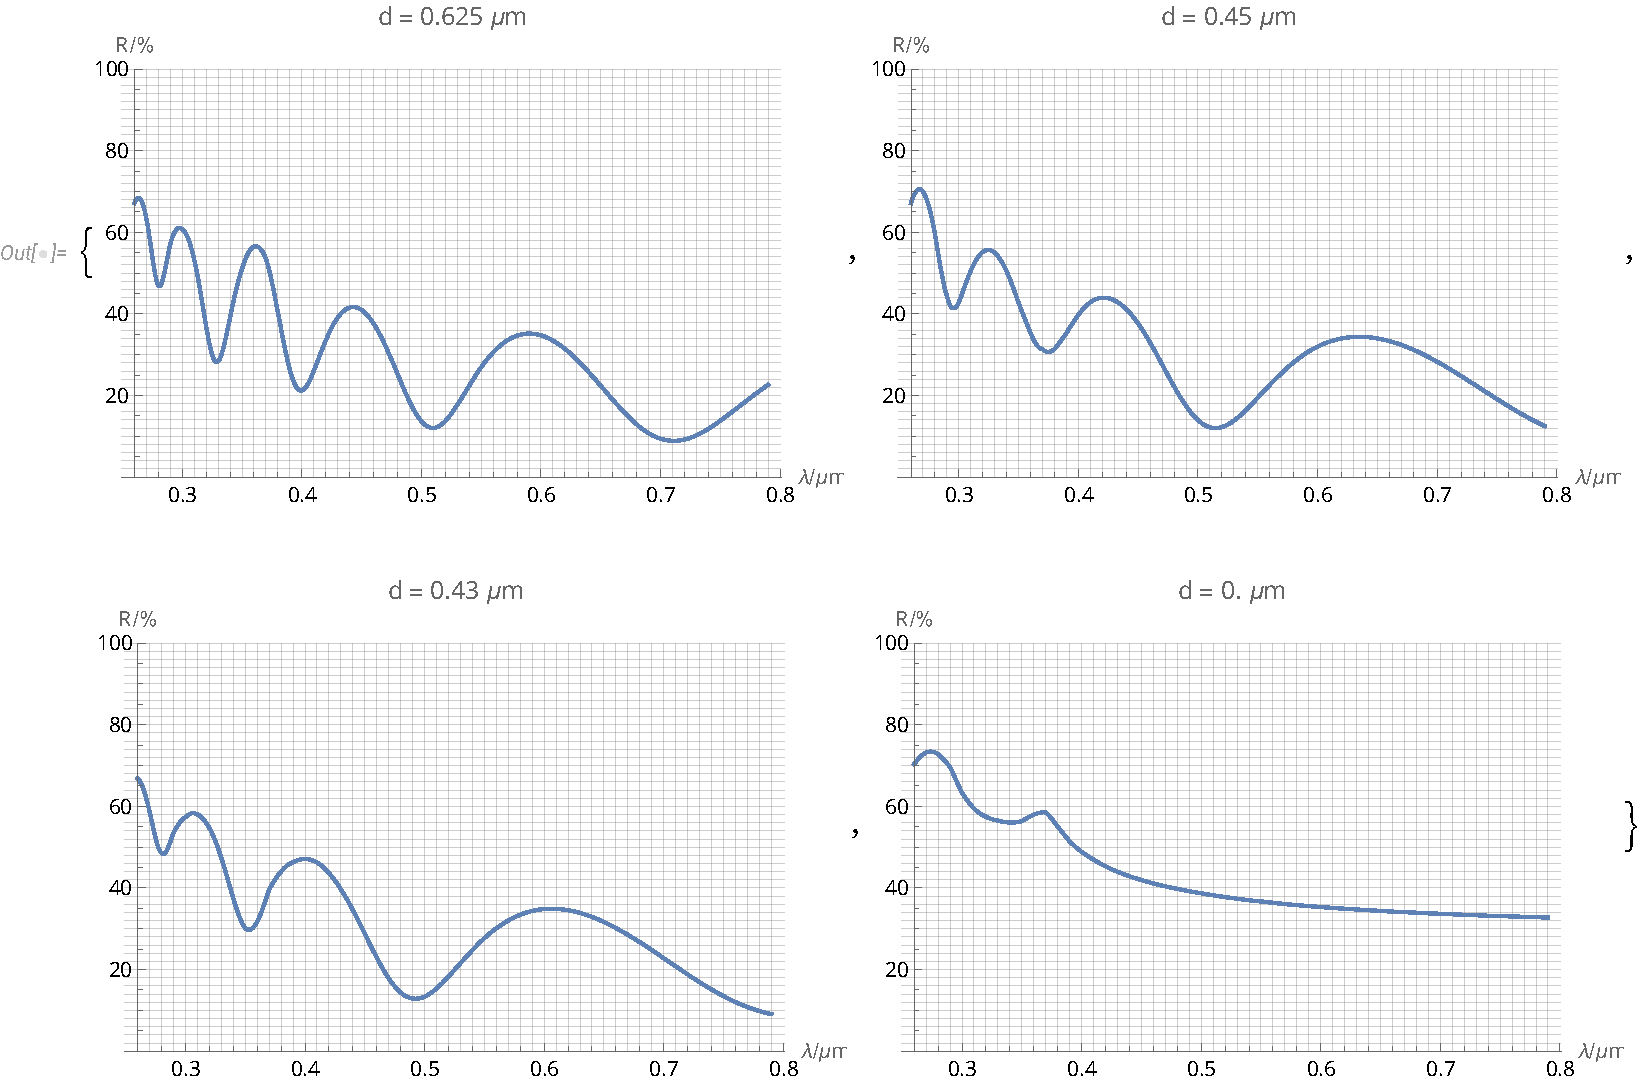
\includegraphics[scale=0.39]{CV/figs/3.2.pdf}
    \end{figure}
\end{frame}

\section{Honors \& Awards}
\begin{frame}{Honors \& Awards}
    \begin{enumerate}
        \item 2021-2022 学年河海大学“优秀学生标兵” \hfill \textit{2022.11}
        \item 河海大学 2021-2022 学年学业优秀奖学金 \hfill \textit{2022.11}
        \item 河海大学 2021-2022 学年科技创新奖学金 \hfill \textit{2022.11}
        \item 河海大学 2021-2022 学年精神文明奖学金 \hfill \textit{2022.11}
        \item 河海大学 2020-2021 学年学业优秀奖学金 \hfill \textit{2021.11}
        \item 河海大学 2020-2021 学年科技创新奖学金 \hfill \textit{2021.11}

              \medskip \hrule \medskip

        \item 江苏省高等学校第二十届高等数学竞赛本科一级A组\ \textit{二等奖} \hfill \textit{2023.06}
        \item 2022年第八届全国大学生物理实验竞赛\ \textit{二等奖}  \hfill \textit{2022.12}
        \item 二零二二年高教社杯全国大学生数学建模竞赛本科组\ \textit{二等奖} \hfill \textit{2022.11}
        \item 江苏省高等学校第十九届高等数学竞赛本科一级A组\ \textit{一等奖} \hfill \textit{2022.11}
        \item 美国大学生数学建模竞赛\textit{Honorable Mention} \hfill \textit{2022}
        \item 第十三届全国大学生数学竞赛(非数学类)\ \textit{一等奖} \hfill \textit{2021.12}
        \item 江苏省高等学校第十八届高等数学竞赛本科一级A组\ \textit{一等奖} \hfill \textit{2021.06}
    \end{enumerate}
\end{frame}

\section{Social Performance}
\begin{frame}{Social Performance}
    \begin{description}
        \item[2020 - 2023:] Blood donations totaled 1700 mL for six times
        \item[2020 - 2022:] Excellent volunteer in the epidemic(COVID-19) prevention, \textit{Linzhang, Handan, Hebei}
        \item[2020:] Volunteer in Jiulong Lake Reading Center, \textit{Jiangning, Nanjing, Jiangsu}
    \end{description}
\end{frame}

\begin{frame}{Epilogue}
    \begin{center}
        {\Huge \calligra Thank you for listening.}

        \vspace{5em}

        Feng Zhe / 冯哲
    \end{center}
\end{frame}

\end{document}